\documentclass{article}
\usepackage{fancyhdr}
\usepackage{extramarks}
\usepackage{amsmath}
\usepackage{amsthm}
\usepackage{amsfonts}
\usepackage{tikz}
\usepackage[plain]{algorithm}
\usepackage{algpseudocode}

\begin{document}
\author{Chuan Lu}
\title{PHYS:5905 Homework 2}
\maketitle

\medskip

\begin{enumerate}

\item
Larmor Motion in constant, uniform magnetic field with zero electric field.

\begin{enumerate}
\item
Figure \ref{problem 1.1} shows the plots of $x(t)$, where the numerical solution is computed with $N=2000$ timesteps:
\begin{figure}[h]
\centering
\vbox{
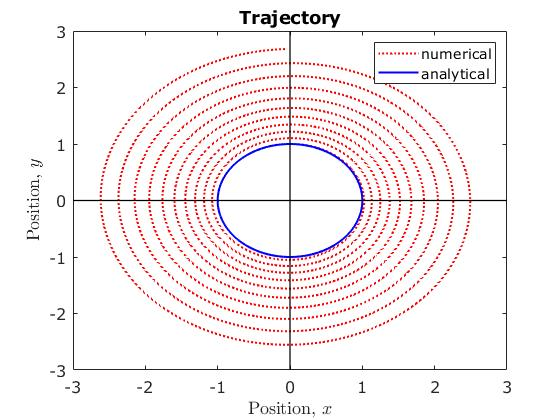
\includegraphics[scale=0.6]{problem1/trajectory_timestep_2000.jpg}
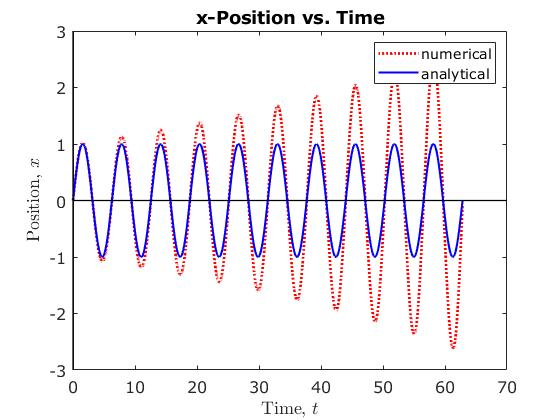
\includegraphics[scale=0.6]{problem1/xposition_timestep_2000.jpg}
}
\caption{The trajectory in the $(x, y)$ plane (top) and the position $x$ as function of time $t$ (bottom). The dot lines are numerical solutions solved with $N=2000$ timesteps and the solid lines are the analytical solutions.}
\label{problem 1.1}
\end{figure}

\item
Figure \ref{problem 1.2} is the error plot with respect to the number of timesteps. The slope is $k = -1.00393$.
\begin{figure}[h]
\centering
\vbox{
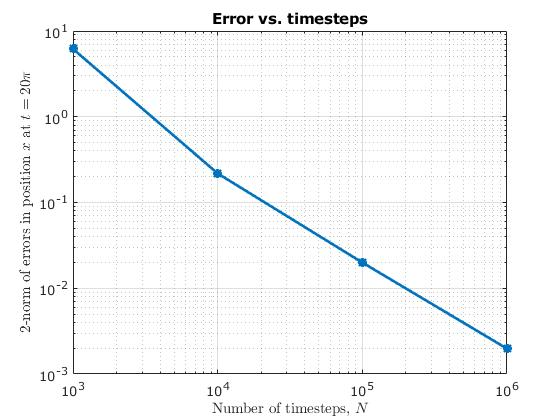
\includegraphics[scale=0.6]{problem1/error.jpg}
}
\caption{The error at $t = 20\pi$ with respect to the number of timesteps $N$.}
\label{problem 1.2}
\end{figure}

\end{enumerate}

\item
$E\times B$ drift in a constant, uniform magnetic and perpendicular electric field.

\begin{enumerate}
\item
Figure \ref{problem 2.1} shows the plots of $x(t)$, where the numerical solution is computed with $N=2000$ timesteps:
\begin{figure}[h]
\centering
\vbox{
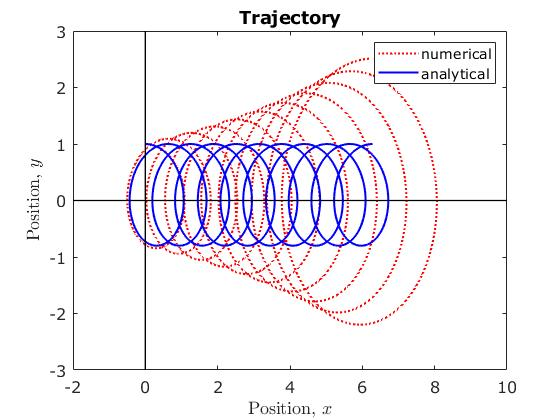
\includegraphics[scale=0.6]{problem2/trajectory_timestep_2000.jpg}
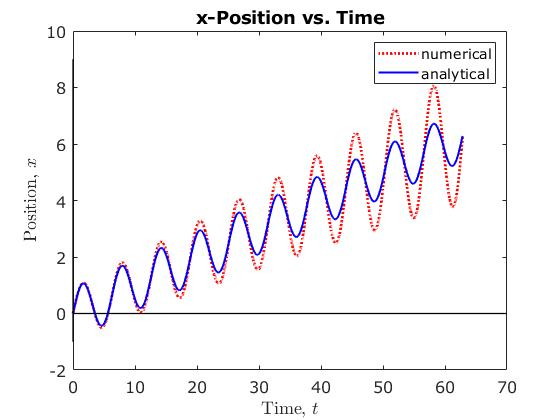
\includegraphics[scale=0.6]{problem2/xposition_timestep_2000.jpg}
}
\caption{The trajectory in the $(x, y)$ plane (top) and the position $x$ as function of time $t$ (bottom). The dot lines are numerical solutions solved with $N=2000$ timesteps and the solid lines are the analytical solutions.}
\label{problem 2.1}
\end{figure}

\item
Figure \ref{problem 2.2} is the error plot with respect to the number of timesteps. The slope is $k = -1.00389$.
\begin{figure}[h]
\centering
\vbox{
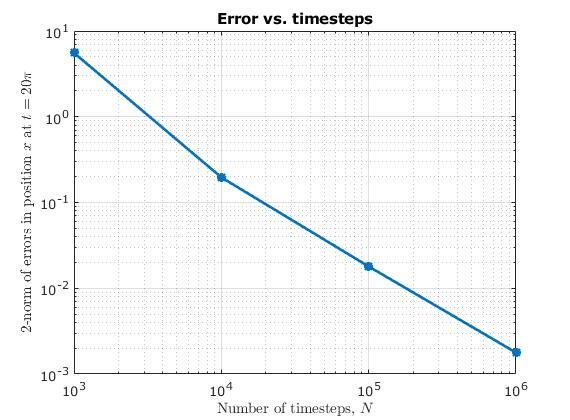
\includegraphics[scale=0.6]{problem2/error.jpg}
}
\caption{The error at $t = 20\pi$ with respect to the number of timesteps $N$.}
\label{problem 2.2}
\end{figure}

We notice that the slopes in both problems are just the same when the number of timesteps $N$ is large enough. This shows that the forward difference method is asymptotically linear.

\end{enumerate}

\item Second-order timestepping for $E\times B$ drift.
\begin{enumerate}
\item
Figure \ref{problem 2b.1} shows the plots of $x(t)$, where the numerical solution is computed with $N=1000$ timesteps and with leapfrog method:
\begin{figure}[h]
\centering
\vbox{
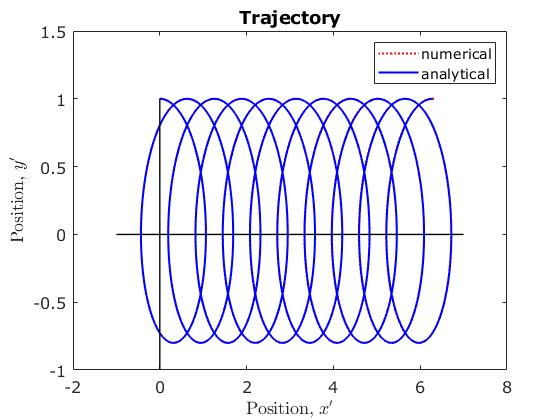
\includegraphics[scale=0.6]{problem2b/trajectory_timestep_1000.jpg}
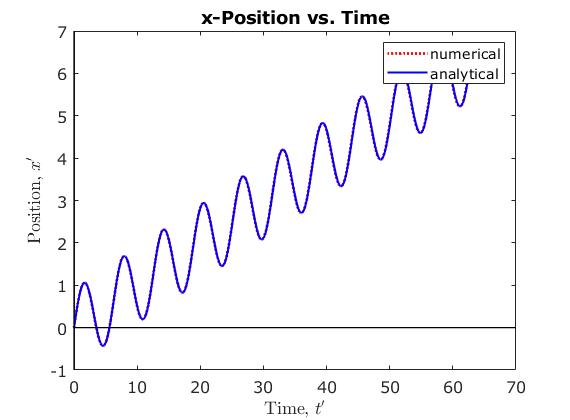
\includegraphics[scale=0.6]{problem2b/xposition_timestep_1000.jpg}
}
\caption{The trajectory in the $(x, y)$ plane (top) and the position $x$ as function of time $t$ (bottom). The dot lines are numerical solutions solved with $N=1000$ timesteps and the solid lines are the analytical solutions.}
\label{problem 2b.1}
\end{figure}

\item
Figure \ref{problem 2b.2} is the error plot with respect to the number of timesteps. The slope is $k = -2$.
\begin{figure}[h]
\centering
\vbox{
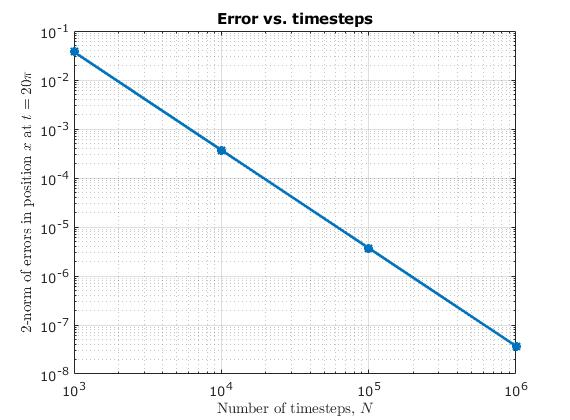
\includegraphics[scale=0.6]{problem2b/error.jpg}
}
\caption{The error at $t = 20\pi$ with respect to the number of timesteps $N$.}
\label{problem 2b.2}
\end{figure}
\end{enumerate}

\item Use Taylor expansion to demonstrate the order of Leapfrog method

In fact, consider the equation
\begin{equation}
\frac{dx}{dt} = v.
\end{equation}
The Taylor expansion at $x_{j} $ leads to
\begin{equation}
x_{j+1} = x_{j} + v_j\Delta t + \frac{1}{2}v'(t_j)(\Delta t)^2 + O((\Delta t)^3 ),
\end{equation}
and
\begin{equation}
x_{j-1} = x_{j} - v_j\Delta t + \frac{1}{2}v'(t_j)(\Delta t)^2 + O((\Delta t)^3 ).
\end{equation}
Hence
\begin{equation}
x_{j+1}-x_{j-1} = 2v_j\Delta t + O((\Delta t)^3 ),
\end{equation}
and we get
\begin{equation}
v_j = \left.\frac{dx}{dt}\right|_{t = t_j} = \frac{x_{j+1}-x_{j-1}}{2\Delta t} + O((\Delta t)^2 ).
\end{equation}


\end{enumerate}


\end{document}T0 = 0; T = 20*pi;
N = 1000;
dt = (T-T0)/N;
q = 1; m = 1;
x0 = [0, 1, 0]'; v0 = [1, 0, 0]';
B0 = 1;

% Normalization
Omega = q*B0/m;
vp = sqrt(v0(1)*v0(1)+v0(2)*v0(2));
r_L = vp/Omega;
x0 = x0/r_L;
v0 = v0/vp;
T0 = T0*Omega;
T = T*Omega;
dt = dt*Omega;

B = @(x, t) B0*[0, 0, 1]';
E = @(x, t) 0.1*vp*B0*[0, 1, 0]';


[x, v, t] = larmor_motion_dimensionless_solver(E, B, x0, v0, T0, T, dt, 2);
[xt, vt, tt] = larmor_motion_analytical_2(N);